
\section{Analog Filters}

\par \indentt Say we have a continuous-time function that represents some tone. The complex Fourier coefficients of that function are the amplitudes of the pure tones that constitute the tone. To turn the tone into a new one while preserving the pitch, all we must do is find those amplitudes (i.e. apply the Fourier approximation), change them, and go back to a continuous-time function (i.e. set the new amplitudes as the coefficients of $\FNT$). This process is diagrammed in Figure \ref{fig:analog_filter_space_diagram}.

\par \bigskip A linear function $s: \VNT \rightarrow \VNT$ will do what we want when \textit{all the pure tones in $\FNT$ are eigenvectors of $s$}. Recall that putting an eigenvector through $s$ returns that same eigenvector, but scaled by some constant (also known as its eigenvalue). From this, a definition for analog filters arises:

\begin{definition}
    An analog filter is a linear function $s: \VNT \rightarrow \VNT$ such that, for all pure tones $e^{\frac{2\pi int}{T}}$, $-N\le n\le N$, $$s(e^{\frac{2\pi int}{T}})=\lambda_s\bigg(\frac{n}{T}\bigg)e^{\frac{2\pi int}{T}}$$
    where $\lambda_s(\frac{n}{T})$ is the \textbf{frequency response} of $s$ with respect to frequency $\frac{n}{T}$.\cite{Ryan}
    \label{defn:analog_filter}
\end{definition}

Applying the filter $s$ to each pure tone in the $N$'th-order complex Fourier series and then summing the results is equivalent to multiplying each element of the frequency response vector $\lambda_s = \{\lambda_s(0),\lambda_s(\frac{1}{T}),\lambda_s(\frac{2}{T}),...,\lambda_s(\frac{n}{T}),...,\lambda_s(\frac{N-1}{T})\}$ by $\FNT$.\footnote{Note that $\lambda_s$ gives the coordinates of $s$ in $\VNT$ under the basis $\FNT$, meaning $s\in\VNT$ and so must itself be some tone of the note with fundamental frequency $\frac{1}{T}$.}

\begin{figure}[h]
    \centering
    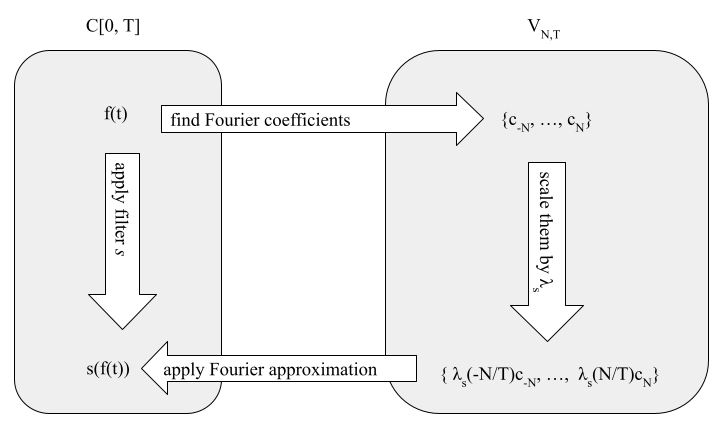
\includegraphics[scale=.35]{analog_filter_space_diagram.png}
    \caption{Moving within and between continuous time and the frequency space}
    \label{fig:analog_filter_space_diagram}
\end{figure}

\subsection{Properties of Analog Filters}

\par \indentt Filters have a few key properties that allow them to aid music production.\cite{Ryan}

\begin{itemize} 
    \item \textit{The composition of multiple filters is itself a filter.} In other words, for any sequence of filters applied one after the other, one can find a single filter that is equivalent to the entire sequence.
    \begin{itemize}
        \item Additionally, \textit{the frequency response for the composition of multiple filters is equal to the product of the frequency responses of the constituent filters.} That means for arbitrary filters $s_1$ and $s_2$, $\lambda_{s_1s_2}(\frac{n}{T}) = \lambda_{s_1}(\frac{n}{T}) \lambda_{s_2}(\frac{n}{T})$.
    \end{itemize}
    \item \textit{Filters commute.} In other words, the order of application does not change the sound that is ultimately produced. Also, if we apply one filter, apply a second, then remove the first, we get the same sound as if we had only applied the second.
\end{itemize}

\begin{theorem}
    The set of filters has the above properties and therefore qualifies as a commutative algebra.

    \begin{proof}
        Consider arbitrary filters $s_1$ and $s_2$ with frequency responses $\lambda_{s_1}(\frac{n}{T})$ and $\lambda_{s_2}(\frac{n}{T})$. We see that
        
        \begin{multline*}
            s_1\left(s_2\left(\puretone{nt}{T}\right)\right) = s_1\left(\lambda_{s_2}\left(\frac{n}{T}\right)\puretone{nt}{T}\right) = \lambda_{s_2}\left(\frac{n}{T}\right)\left(s_1\left(\puretone{nt}{T}\right)\right) \\= \lambda_{s_2}\left(\frac{n}{T}\right)\lambda_{s_1}\left(\frac{n}{T}\right)\left(\puretone{nt}{T}\right) \\= \lambda_{s_2}\left(\frac{n}{T}\right)\left(\lambda_{s_1}\left(\frac{n}{T}\right)\puretone{nt}{T}\right) = \lambda_{s_2}\left(\frac{n}{T}\right)s_1\left(\puretone{nt}{T}\right) = s_2\left(s_1\left(\puretone{nt}{T}\right)\right).
        \end{multline*}
        
        Therefore, $s_1$ and $s_2$ commute. Additionally, since the composition of $s_1$ and $s_2$ is equal to $\lambda_{s_2}(\frac{n}{T})\lambda_{s_1}(\frac{n}{T})(\puretone{nt}{T})$, it is a filter with frequency response $\lambda_{s_1}(\frac{n}{T}) \lambda_{s_2}(\frac{n}{T})$.
    \end{proof}
\end{theorem}

\newpage

\subsection{Example: Low-Pass and High-Pass Filters}

\par \indentt Two of the most commonly-used types of filter are called \textbf{low-pass filters (LPFs)} and \textbf{high-pass filters (HPFs)}. Low-pass filters remove pure tones with frequencies above some threshold and allow the frequencies below it to pass through. High-pass filters do the opposite.

\par \bigskip To see how this works, consider the signal $f(t) = \puretone{(1)t}{T} + \puretone{(2)t}{T} + \puretone{(3)t}{T} + \puretone{(4)t}{T} + \puretone{(5)t}{T} + \puretone{(6)t}{T}$. This function is the sum of the pure tones with frequency $\frac{n}{T},~1 \le n \le 6$, and its Fourier coefficients are clearly $\{0,1,1,1,1,1,1\}$. Figure \ref{fig:5th_order_tone} shows an amplitude-over-time graph of the tone represented by this signal and its constituent pure tones.

\begin{figure}[h]
    \centering
    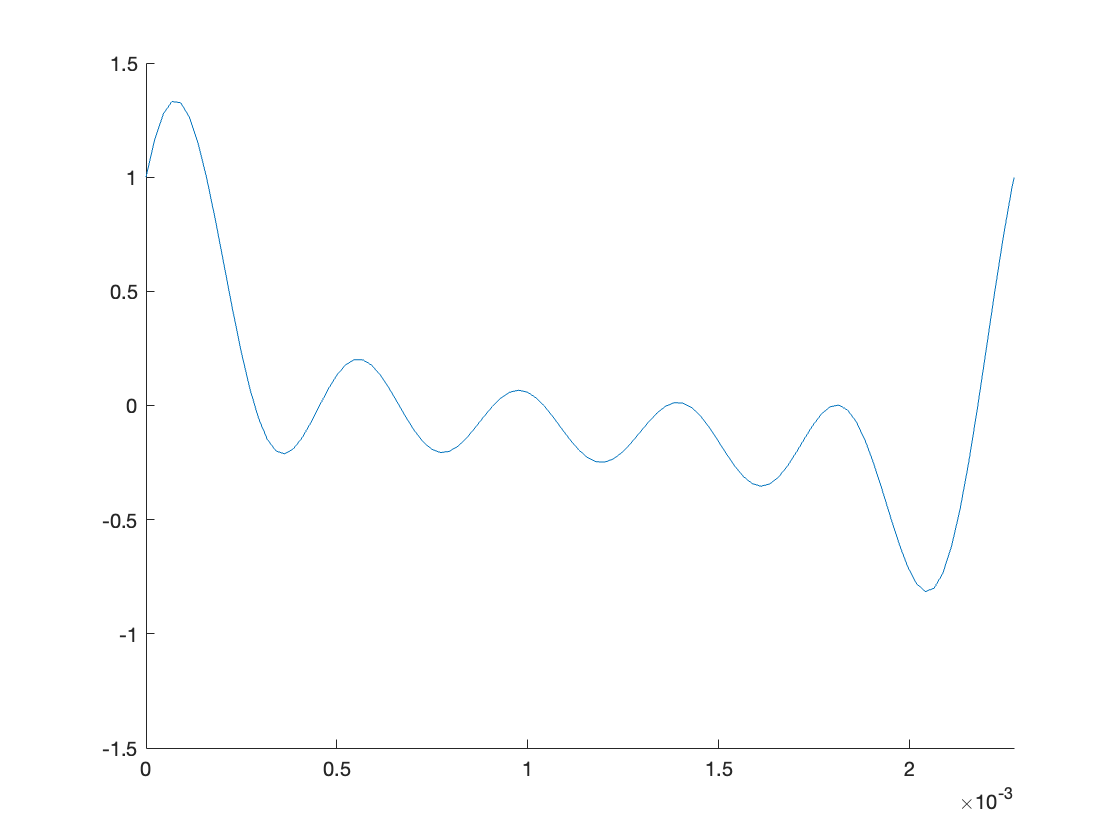
\includegraphics[scale=.15]{6th_order_tone.png}
    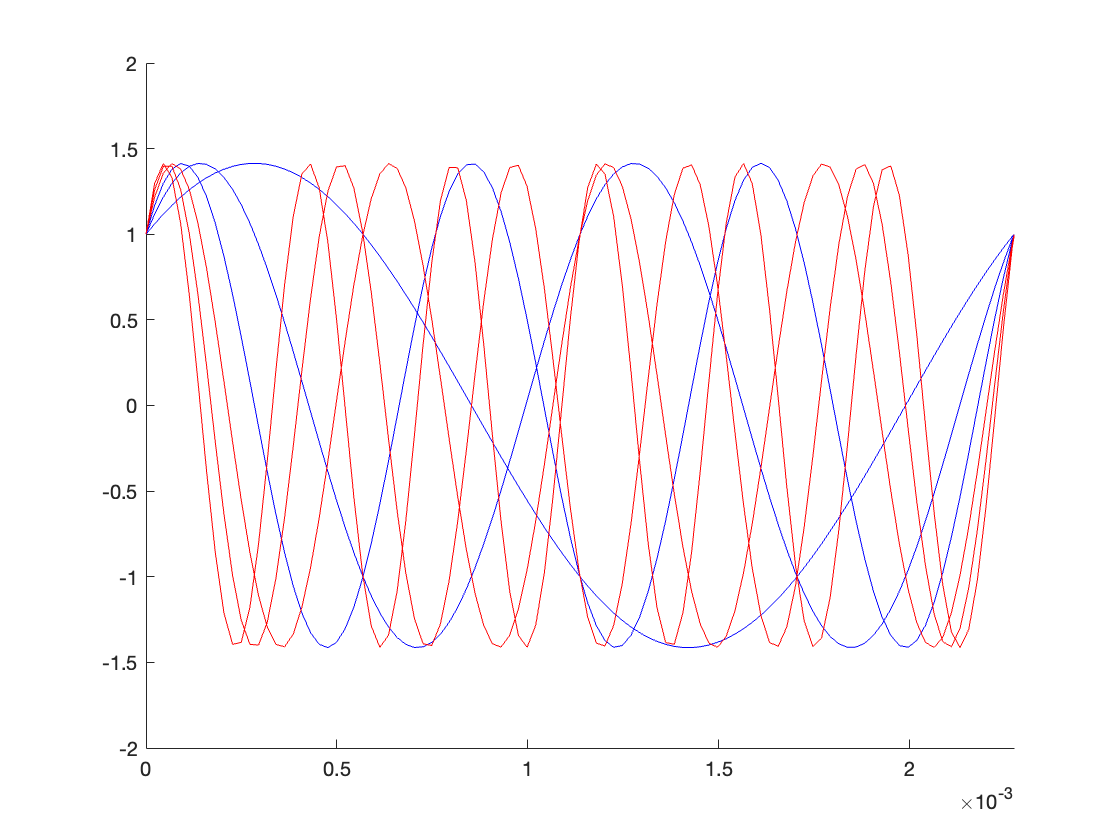
\includegraphics[scale=.15]{6th_order_tone_cluster.png}
    \caption{A sixth-order tone and its constituent pure tones}
    \label{fig:5th_order_tone}
\end{figure}

\par \bigskip When the LPF is applied, the amplitudes of the three higher pure tones ($n\in\{1,2,3\}$, shown in red) are set to 0, while the three lower pure tones ($n\in\{4,5,6\}$, shown in blue) are left alone. The HPF removes the lower and keeps the higher.


$$\lambda_{LPF} = \{0,1,1,1,0,0,0\} \hspace{.5in} \lambda_{HPF} = \{0,0,0,0,1,1,1\}$$


\begin{figure}[h]
    \centering
    \begin{tabular}{cc}
        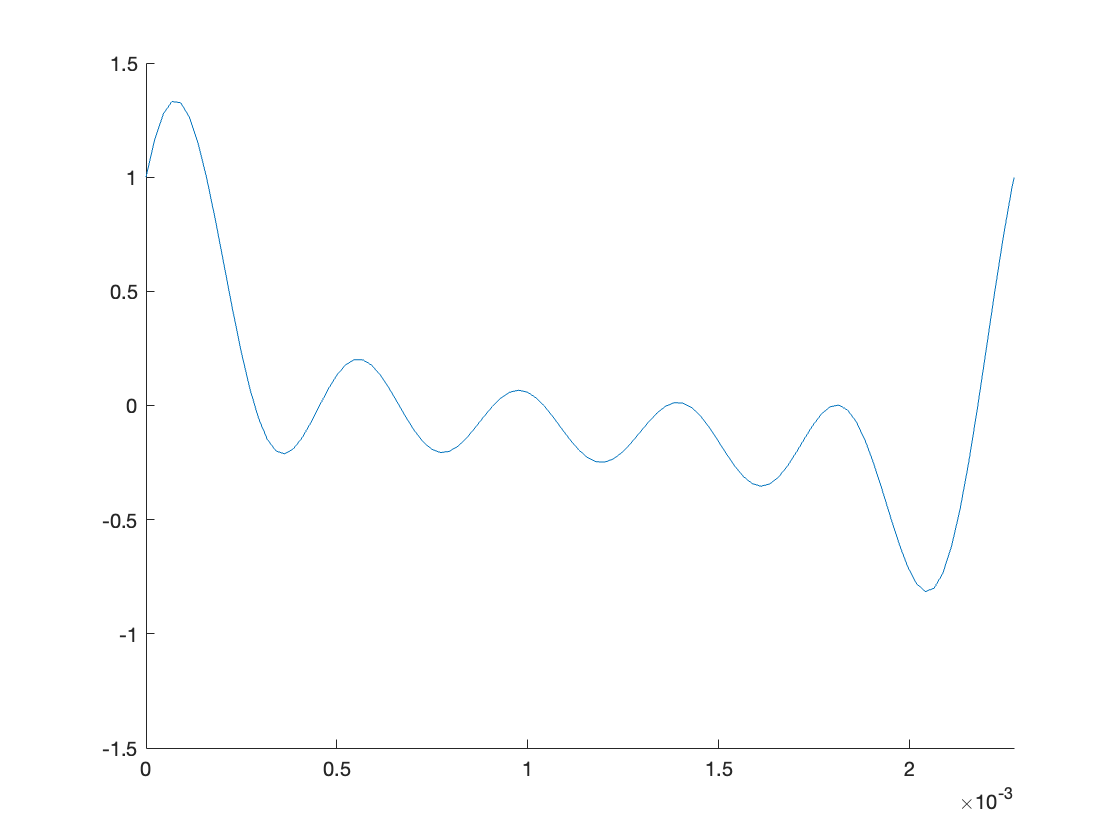
\includegraphics[scale=.15]{6th_order_tone.png} & 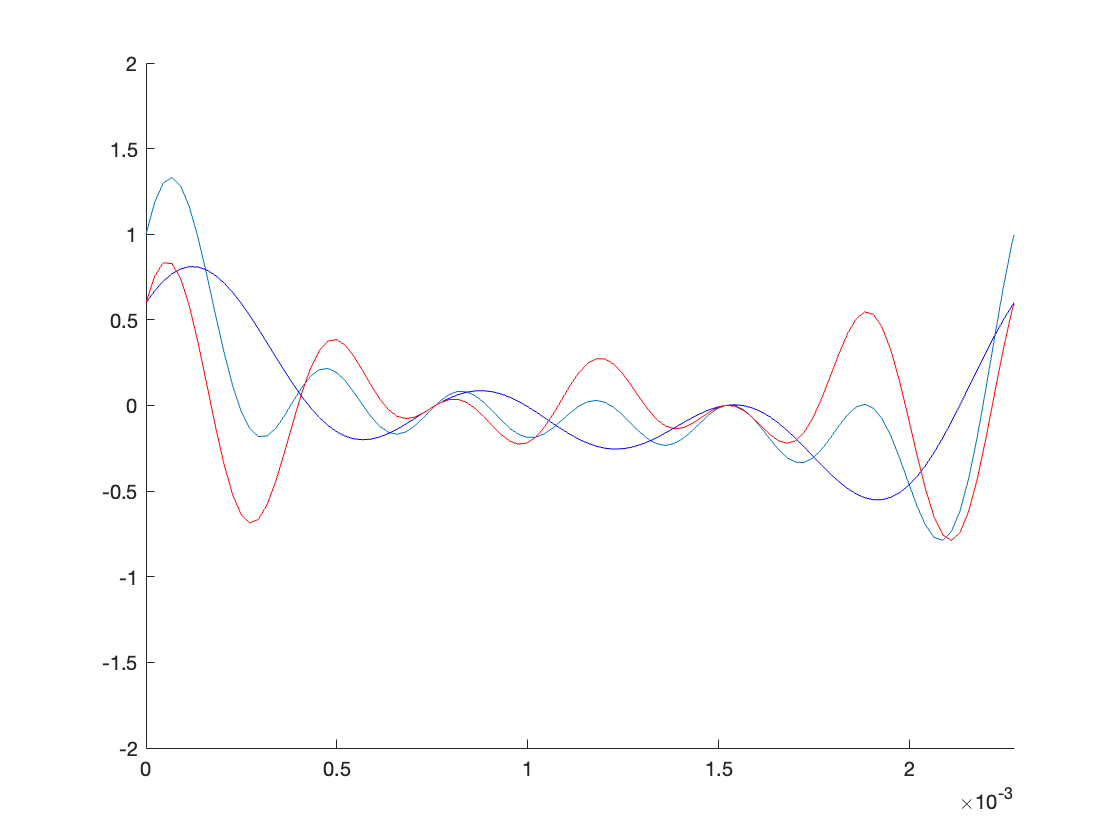
\includegraphics[scale=.15]{6th_order_tone_LPF_HPF.png}\\
        \href{https://drive.google.com/file/d/18jKNvtlR9ocDlZKemNlN8vrQi96WZRs7/view?usp=sharing}{\color{blue} $[\blacktriangleright]$ Unfiltered tone}\\
        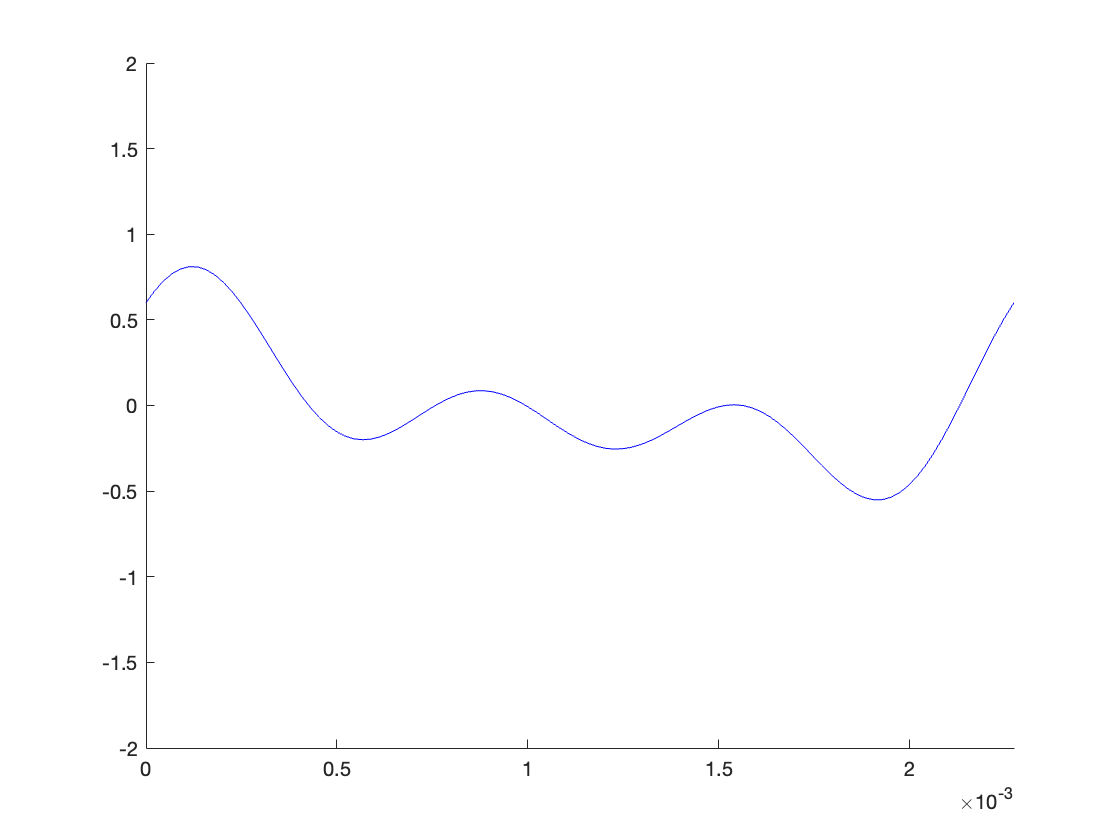
\includegraphics[scale=.15]{6th_order_tone_LPF.png} & 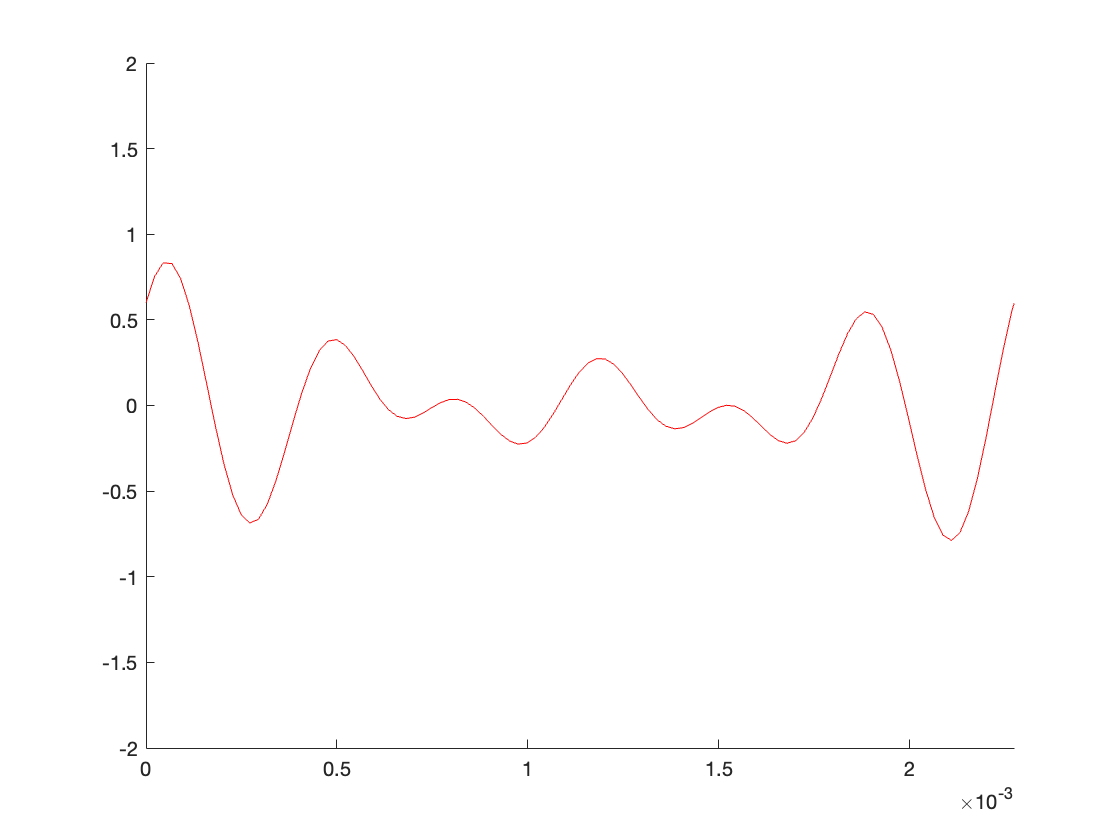
\includegraphics[scale=.15]{6th_order_tone_HPF.png}\\
        \href{https://drive.google.com/file/d/1tjxLPXLkrhaWuaD99JjpF7ysoxVjJbhO/view?usp=sharing}{\color{blue} $[\blacktriangleright]$ Tone after LPF is applied} & \href{https://drive.google.com/file/d/1M0l6kBrHJ0WfIffrrLXCgEpl2vRaUZTi/view?usp=sharing}{\color{blue} [$\blacktriangleright$] Tone after HPF is applied}\\
    \end{tabular}
    \caption{The LPF and HPF applied to a basic sixth-order tone}
    \label{fig:5th_order_tone_filtered}
\end{figure}

\par \bigskip Listen to the audio files linked in Figures \ref{fig:5th_order_tone} and \ref{fig:5th_order_tone_filtered} to hear the effect of these two filters on our sixth-order pure tone. The LPF produces a more gentle and well-rounded tone, while the HPF produces a tinnier, more aggressive tone.

\par \bigskip 